\documentclass[11pt,a4paper]{article}
\usepackage[utf8]{inputenc}
\usepackage[spanish,es-tabla]{babel}
\usepackage{amsmath}
\usepackage{amsfonts}
\usepackage{amssymb}
\usepackage{graphicx}
\usepackage{float}

\usepackage{vmargin}

\setpapersize{A4}
\setmargins{2.5cm}              % margen izquierdo
{1.5cm}                         % margen superior
{16.5cm}                        % anchura del texto
{23.42cm}                       % altura del texto
{10pt}                          % altura de los encabezados
{1cm}                           % espacio entre el texto y los encabezados
{0pt}                           % altura del pie de página
{2cm}                           % espacio entre el texto y el pie de página

\title{ 
    Emisión de titulos universitarios
    en la Blockchain
}
\author{
    Saez, Lautaro Andres \\ \small{ LautaroAndresSaez@gmail.com } 
    \and 
    Riperto, Adriel Aaron \\ \small{ aaron.ariperto@gmail.com } 
}
\date{\today}

\begin{document}
    \maketitle

    \section{Introducción}

    \section{Estado del arte}

        Esta sección tiene como objetivo tratara el estado actual de la tematica a abordar.
        En general debido a que blockchain se encuentra en constante crecimiento, no hay 
        grandes aplicaciones implementadas en el ambito de titulos academicos, sino que existen
        trabajos que proponen modelos a implementar. %Correguir implementaciones!

        \subsection{Blockchain federal Argentina}

        En primer lugar desde la pagina web de la Blockchain federal  Argentina %Incluir referencia a la BFA 
        se menciona este trabajo como una posible aplicación nombrando las 
        ventajas que este tiene las cuales son:
        
        \begin{itemize}
            \item Garantiza que no sea posible alterar la 
            información de las actas sin que esa modificación sea detectada y así aumenta la confianza en la autenticidad de los títulos emitidos. 
            \item Transparencia en el proceso de digitalización.
            \item Permite un contexto de confianza entre organismos y partes interesadas. 
            \item Auditable.
            \item Permite demostrar que no existen actos de negligencia (títulos truchos) en torno a la emisión de títulos.
            \item Se podría dar diferentes vigencias a certificado de títulos en trámite, o similares, certificadas en la blockchain.
        \end{itemize}

        Por otro lado se proponen posibles mejoras a esta implementación creando un portafolios digital, lo cual 
        permitiria modificar los permisos de acceso.

        \begin{figure}
            \centering
            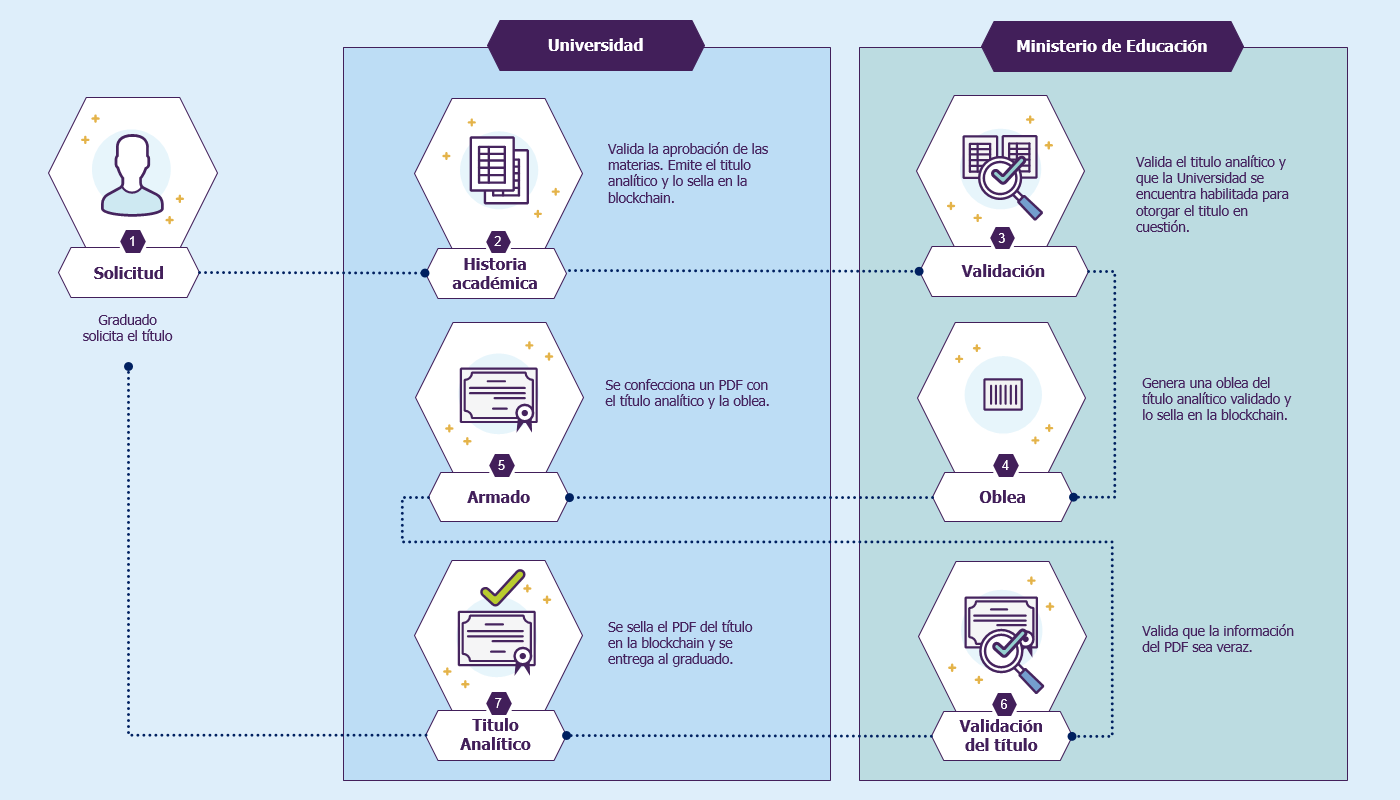
\includegraphics[width=\textwidth]{Img/cuadro_problematica.png}
            \caption{}
            \label{fig:cuadro_problematica}
        \end{figure}

        \subsection{AWS example}
    \section{Objetivos}

        \subsection{Objetivo principal}

        Implementar las bases de un sistema en la blockchain que permita la generacion 
        y autenticacion de los titulos universitarios. 
        
        \subsection{Objetivos secundarios}

        \begin{itemize}
            \item Analizar los procesos que implican la generacion y validacion de un titulo.
            \item Evaluar el ecosistema de tecnologias a implementar.
            \item Diseñar los componentes de la aplicaciones.
            \item Implementar el sistema utilizando la BFA. 
        \end{itemize}


    \section{Desafíos}

        Esta seccion tiene como objetivo describir los desafios que se deben afrontar para poder realizar la aplicacion propuesta.

        \subsection{Modelo y procesos del negocio} 

            El primer desafio planteado implica analizar y comprender por parte del equipo, los procesos que implican la 
            generacion y validacion de un titulo universitario. Esto tiene como objetivo replicar y mejorar los procesos 
            en el sistema a construirse.
        
        \subsection{Aprendizaje de tecnologias} 

            El segundo desafio sera aprender las siguientes tecnologias:
            
            \begin{itemize}
                \item Blockchain Federal Argentina
                \item React
                \item NodeJS
            \end{itemize}
            
            Las tecnologias planteadas tienen como objetivo crear una arquitectura viable y limpia para el desarrollo del sistema.
            
            
        \subsection{Difusion del sistema} 

            Por ultimo se debe realizar una difusion del ecosistema planteado y lograr una aceptacion por parte de los alumnos y las diferentes entidades.
            El objetivo de este desafio es lograr una mejora en la gestion de titulos, eliminando los intermediarios y facilitando la accesibilidad 
            a los documentos universitarios. 

    \section{Etapas}

        La forma de trabajo a llevar a cabo sera la siguiente:

        \begin{table}[H]
            \centering
            \begin{tabular*}{|c|c|}
                \hline Activdad & Tiempo estimado \\ 
                \hline Prueba de concepto en la BFA & \\
                \hline Planificacion de los smart contracts & \\
                \hline Analisis & \\
                \hline Diseño de la arquitectura & \\ 
                \hline Desarrollo de los smart contracts & \\
                \hline Desarrollo del backend & \\ 
                \hline Desarrollo del frontend & \\ 
                \hline Despliegue sobre BFA & \\
                \hline Tiempo total & \\
            \end{tabular*}
            \label{tab:etapas}
        \end{table}

 
    \section{Conclusiones}

\end{document}